% Created 2020-05-24 Sun 16:45
% Intended LaTeX compiler: pdflatex
\documentclass[presentation]{beamer}
\usepackage[utf8]{inputenc}
\usepackage[T1]{fontenc}
\usepackage{graphicx}
\usepackage{grffile}
\usepackage{longtable}
\usepackage{wrapfig}
\usepackage{rotating}
\usepackage[normalem]{ulem}
\usepackage{amsmath}
\usepackage{textcomp}
\usepackage{amssymb}
\usepackage{capt-of}
\usepackage{hyperref}
\usepackage{minted}
\usepackage[utf8]{inputenc}
\usepackage{color}
\usetheme[height=7mm]{Rochester}
\setbeamertemplate{footline}[frame number]
\usecolortheme[accent=red, light]{solarized}
\setbeamercolor{frametitle}{bg=solarizedRebase02,fg=solarizedAccent}
\setbeamercolor{author in head/foot}{bg=solarizedRebase02,fg=solarizedRebase01}
\setbeamercolor{title in head/foot}{bg=solarizedRebase02,fg=solarizedRebase01}
\setbeamercolor{block title}{bg=solarizedRebase0,fg=solarizedRebase02}
\setbeamercolor{block body}{bg=solarizedRebase02,fg=solarizedRebase0}
\setbeamercolor{item}{bg=solarizedRebase02,fg=solarizedAccent}
\beamertemplatenavigationsymbolsempty
\usemintedstyle{manni}
\AtBeginSection[]{
\begin{frame}
\vfill
\centering
\begin{beamercolorbox}[sep=8pt,center,shadow=true,rounded=true]{title}
\Huge\insertsectionhead\par%
\end{beamercolorbox}
\vfill
\end{frame}
}
\usetheme{default}
\author{Sebastian Stabinger}
\date{SS2020}
\title{Einführung in C++, Namespaces und Ein-/Ausgabe}
\hypersetup{
 pdfauthor={Sebastian Stabinger},
 pdftitle={Einführung in C++, Namespaces und Ein-/Ausgabe},
 pdfkeywords={},
 pdfsubject={},
 pdfcreator={Emacs 26.3 (Org mode 9.1.9)}, 
 pdflang={Ger}}
\begin{document}

\maketitle

\section{Hintergründe von C++}
\label{sec:orga98b9bb}
\begin{frame}[label={sec:org4cffd0f}]{Zeitleiste}
\begin{columns}
\begin{column}{0.5\columnwidth}
\begin{description}
\item[{1979}] Arbeit an "C with classes" beginnt
\item[{1983}] Umbenennung in C++
\item[{1998}] Erster ISO C++ Standard
\item[{2011}] \alert{Neuer ISO C++ Standard}
\item[{2014}] Minor Revision
\item[{2017}] Major Revision
\item[{2020}] Major Revision
\end{description}
\end{column}
\begin{column}{0.5\columnwidth}
\begin{center}\begin{figure}[htbp]
\centering
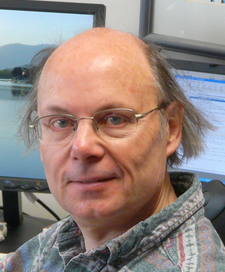
\includegraphics[width=0.7\textwidth]{data/ae/50aadc-3e16-4ac9-9f73-cf048cdfa434/screenshot-20160217-143616.png}
\caption{Bjarne Stroustrup. Erster Entwickler von C++}
\end{figure}\end{center}
\end{column}
\end{columns}
\end{frame}
\begin{frame}[label={sec:org232c96f}]{Abhängigkeiten}
\begin{center}\begin{figure}[htbp]
\centering
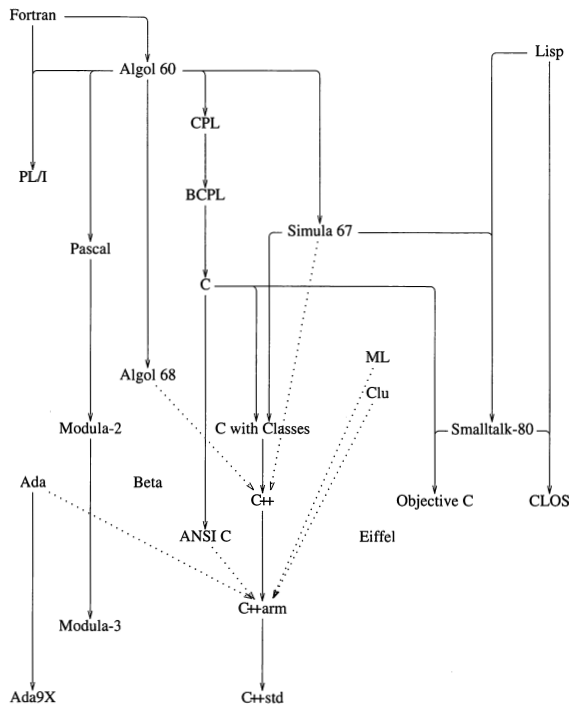
\includegraphics[height=0.8\textheight]{data/2b/515ad4-e3c4-4834-a7be-e95147807c04/screenshot-20160217-144741.png}
\caption{Abhängigkeiten von C++}
\end{figure}\end{center}
\end{frame}
\begin{frame}[fragile,label={sec:org565996e}]{Warum C++?}
 \begin{itemize}
\item Sehr \alert{schnell}
\item \alert{Hardwarenahe Programmierung} ist möglich
\item Problemloses verwenden von \alert{C-Libraries}
\item \alert{Flexibel}: Vom Microcontroller über Spiele bis zum High Performance
Cluster.
\item Im Gegensatz zu C ist auch ein \alert{hohes Maß an Abstraktion} möglich
(OOP, Templates, Meta Template Programming, \ldots{}). Das macht das
Programmieren letztlich \alert{einfacher}.
\item \alert{Grössere Standardbibliothek} (aber immer noch klein im Vergleich zu
Java, Python, C\#, etc.) (Container, {\color{solarizedYellow}\texttt{all\_of}}, {\color{solarizedYellow}\texttt{find}}, \ldots{})
\item Existiert seit \alert{35 Jahren} und wird auch weiterhin seinen Platz haben
\item \alert{Große Code Base} (Fast alle Anwendungsprogramme sind z.B. in C++
geschrieben)
\end{itemize}
\end{frame}
\begin{frame}[label={sec:org99f0a8a}]{Was können wir durchmachen?}
\begin{itemize}
\item C++ ist wesentlich komplexer als C
\begin{itemize}
\item C Standardwerk: 270 Seiten
\item C++ Standardwerk: \alert{1400 Seiten!}
\end{itemize}
\item Wenn man C++ so programmiert wie man es Heute verwenden sollte, hat
es nicht mehr sehr viel mit C zu tun.
\begin{itemize}
\item In sehr vielen Firmen wird allerdings auch kein modernes C++
programmiert!
\end{itemize}
\item Wir werden nur Zeit haben uns ein paar Konzepte von C++ anzusehen
und für den Rest werden wir weiter C verwenden!
\begin{itemize}
\item Das ist nicht ideal, aber für mehr reicht die Zeit leider nicht
aus
\end{itemize}
\end{itemize}
\end{frame}
\begin{frame}[fragile,label={sec:org749e845}]{Hello World}
 Zur Erinnerung: Ein Hello World Programm in C:
\begin{block}{C}
\begin{minted}[fontsize=\scriptsize,numberblanklines=false]{c}
#include <stdio.h>
int main() {
  printf("Hello World\n");
}
\end{minted}
\end{block}
Hier das äquivalente Programm in C++:
\begin{block}{C++}
\begin{minted}[fontsize=\scriptsize,numberblanklines=false]{c++}
#include <iostream>
int main() {
  std::cout << "Hello World" << std::endl;
}
\end{minted}
\end{block}
\end{frame}
\section{Ein und Ausgabe}
\label{sec:org43d9c99}
\begin{frame}[fragile,label={sec:org9c64a01}]{\texttt{cout} (\textbf{c}haracter \textbf{out}put)}
 \begin{itemize}
\item Verwendbar nach {\color{solarizedYellow}\texttt{\#include <iostream>}}
\item Dient der \alert{Ausgabe} von Daten auf dem Bildschirm: \newline {\color{solarizedYellow}\texttt{std::cout << <daten>;}}
\item {\color{solarizedYellow}\texttt{cout} }gibt einen Wert \alert{automatisch korrekt} aus. {\color{solarizedYellow}\texttt{\%d, \%f, ...}}
ist nicht notwendig.
\item Ausgaben können durch wiederholtes {\color{solarizedYellow}\texttt{<<} }aneinandergereiht werden.\newline
{\color{solarizedYellow}\texttt{std::cout << "Hello " << "World" << "!\textbackslash{}n";}}
\item {\color{solarizedYellow}\texttt{std::endl} }fügt einen Zeilenumbruch ein. Als Alternative kann auch
{\color{solarizedYellow}\texttt{\textbackslash{}n} }wie in C verwendet werden
\end{itemize}
\begin{block}{Beispiel}
\begin{minted}[fontsize=\scriptsize,numberblanklines=false]{c++}
int a = 23; std::string b = "Bla"; double c = 42.47; char d = 'Z';
std::complex<int> e = {4, 2};

std::cout << a << " " << b << " " << c << " " << d << " " << e;
// Ausgabe: 23 Bla 42.47 Z (4,2)
\end{minted}
\end{block}
\end{frame}

\begin{frame}[fragile,label={sec:org7846ab7}]{\texttt{cin} (\textbf{c}haracter \textbf{in}put)}
 \begin{itemize}
\item Verwendbar nach {\color{solarizedYellow}\texttt{\#include <iostream>}}
\item Dient der \alert{Eingabe} von Daten durch den Benutzer: \newline {\color{solarizedYellow}\texttt{std::cin >> <daten>;}}
\item Weiß wie {\color{solarizedYellow}\texttt{cout} }welcher Datentyp eingelesen werden soll
\end{itemize}
\begin{block}{Beispiel}
\begin{minted}[fontsize=\scriptsize,numberblanklines=false]{c++}
int a; std::string b; double c; char d; std::complex<double> e;
std::cin >> a; // Liest Ganzzahl
std::cin >> b; // Liest String (ohne Leerzeichen)
std::cin >> c; // Liest Fließkommazahl
std::cin >> d; // Liest einzelnes Zeichen
std::cin >> e; // Liest Komplexe Zahl im Format (real, imag)
\end{minted}
\end{block}
\end{frame}
\begin{frame}[fragile,label={sec:org44a55f4}]{Eingabe - Nützliches Tipps}
 \begin{block}{Einlesen einer ganzen Zeile in einen String mit Leerzeichen etc.}
\begin{minted}[fontsize=\scriptsize,numberblanklines=false]{c++}
std::string str;
std::getline(std::cin, str);
\end{minted}
\end{block}
\begin{block}{Eingabebuffer löschen}
\begin{minted}[fontsize=\scriptsize,numberblanklines=false]{c++}
#include <limits>
// ...
std::cin.clear();
std::cin.ignore(std::numeric_limits<std::streamsize>::max())
\end{minted}
\end{block}
\end{frame}
\begin{frame}[fragile,label={sec:orgfa4c589}]{\texttt{cin/cout} - Beispiel}
 \begin{minted}[fontsize=\scriptsize,numberblanklines=false]{c++}
#include <iostream>
#include <string>

int main() {
  std::string vorname;
  std::cout << "Vorname: ";
  std::cin >> vorname;
  std::string nachname;
  std::cout << "Nachname: ";
  std::cin >> nachname;
  int wiederholungen;
  std::cout << "Wiederholungen: ";
  std::cin >> wiederholungen;

  for (int i = 0; i < wiederholungen; i++) {
    std::cout << "Hallo " << vorname << " " << nachname << std::endl;
  }
}
\end{minted}
\end{frame}
\section{Namespaces}
\label{sec:org05c9fbc}
\begin{frame}[fragile,label={sec:org0775f26}]{Namespace - Das Problem in C}
 Namespace auf Deutsch:
\alert{Namensraum} \footnote{\href{https://de.wikipedia.org/wiki/Namensraum}{https://de.wikipedia.org/wiki/Namensraum}}
\begin{block}{Beispiel}
\begin{itemize}
\item Angenommen wir haben zwei Bibliotheken ({\color{solarizedYellow}\texttt{control.h} }und {\color{solarizedYellow}\texttt{cpu.h}})
\item Beide implementieren eine Funktion {\color{solarizedYellow}\texttt{int check\_state();}}
\end{itemize}
\begin{minted}[fontsize=\scriptsize,numberblanklines=false]{c}
#include "control.h"
#include "cpu.h"

if (check_state() == 42) {
  printf("Status ok\n");
}
\end{minted}
\end{block}
Dieser Code wird \alert{nicht funktionieren}. Woher soll der Compiler
wissen, welche der beiden Funktionen {\color{solarizedYellow}\texttt{check\_state} }aufgerufen werden
soll?
\end{frame}
\begin{frame}[fragile,label={sec:orgeb92dcf}]{Namespace - Die Lösung in C++}
 \begin{itemize}
\item C++ löst dieses Problem durch die Einführung sogenannter \alert{Namespaces}
(\alert{Namensräume})
\item Namespaces definieren \alert{benannte Gültigkeitsbereiche} von Funktionen,
Variablen, Klassen, \ldots{}
\item Um von außerhalb eines Namespaces auf dessen Inhalt zugreifen zu
können muss dessen \alert{Name explizit genannt} werden.
\end{itemize}
Das vorherige Beispiel könnte gelöst werden indem die beiden
Funktionen in unterschiedlichen Namespaces deklariert werden
\begin{exampleblock}{Beispiel: Lösung in C++}
\begin{minted}[fontsize=\scriptsize,numberblanklines=false]{c++}
#include "control.h" // Verwendet z.B. den Namespace ccont 
#include "cpu.h" // Verwendet z.B. den Namespace cpu_n

if (cpu_n::check_state() == 42) { std::cout << "CPU ok\n"; }
if (ccont::check_state() == 47) { std::cout << "Controller ok\n"; }
\end{minted}
\end{exampleblock}
\end{frame}
\begin{frame}[fragile,label={sec:org6552fd4}]{Namespace - Deklaration}
 Die Deklaration eines Namespaces folgt dem Muster:

{\color{solarizedYellow}\texttt{namespace <name> \{ <code> \}}}
\begin{block}{Beispiel}
\begin{minted}[fontsize=\scriptsize,numberblanklines=false]{c++}
namespace ccont {
int ok = 47;
int check_state() { return ok; } // Unser Controller is immer OK :-)
} // namespace ccont
\end{minted}
Die Variable {\color{solarizedYellow}\texttt{ok} }und die Funktion {\color{solarizedYellow}\texttt{check\_state} }befinden sich somit
im Namensraum {\color{solarizedYellow}\texttt{ccont}}
\end{block}
\begin{itemize}
\item Ein Namespace muss nicht am Stück deklariert werden. Wir können
jederzeit durch einen neuen {\color{solarizedYellow}\texttt{namespace} }Block einem bereits
existierenden Namensraum \alert{Elemente hinzufügen}. Auch in
\alert{unterschiedlichen Dateien}!
\end{itemize}
\end{frame}
\begin{frame}[fragile,label={sec:org9c05804}]{Namespace - Zugriff}
 Auf Elemente eines Namensraums wird folgendermaßen zugegriffen:
{\color{solarizedYellow}\texttt{<namespace>::<element>}}
\begin{block}{Beispiel}
Wir wollen ausserhalb von {\color{solarizedYellow}\texttt{ccont} }auf die Funktion {\color{solarizedYellow}\texttt{check\_status()}}
zugreifen.
\begin{minted}[fontsize=\scriptsize,numberblanklines=false]{c++}
std::cout << ccont::check_state(); // Gibt 47 zurück
\end{minted}
\end{block}
\begin{block}{Standardnamensraum}
Alle Standardfunktionen von C++ liegen im Namensraum {\color{solarizedYellow}\texttt{std} }(für
Standard).
\end{block}
\end{frame}
\begin{frame}[fragile,label={sec:org6eb249e}]{Namespace - Import}
 Manchmal möchte man den Namespace nicht immer explizit angeben
(besonders beim {\color{solarizedYellow}\texttt{std} }Namensraum üblich)
\begin{block}{{\color{solarizedYellow}\texttt{using}}}
\begin{minted}[fontsize=\scriptsize,numberblanklines=false]{c++}
std::cout << "Hello World!" << std::endl;
using std::cout; // Ab hier können wir einfach cout verwenden
cout << "Hello Simple World!" << std::endl;
\end{minted}
\end{block}
\begin{block}{{\color{solarizedYellow}\texttt{using namespace}}}
\begin{minted}[fontsize=\scriptsize,numberblanklines=false]{c++}
using namespace std; // Ab hier können wir überall std:: weglassen
cout << "Hello Really Simple World!" << endl;
\end{minted}
\end{block}
\begin{itemize}
\item {\color{solarizedYellow}\texttt{using} }importiert ein Element
\item {\color{solarizedYellow}\texttt{using namespace} }importiert den ganzen Namensraum
\item Man muss mit {\color{solarizedYellow}\texttt{using namespace} }vorsichtig sein, da man die ganzen
Vorteile von Namespaces verliert!
\end{itemize}
\end{frame}
\begin{frame}[fragile,label={sec:orgbd64942}]{Namespace - Verschachtelung}
 Ein Namespace kann innerhalb eines anderen Namespaces deklariert
werden. Wir greifen auf verschachtelte Namensräume durch wiederholtes
{\color{solarizedYellow}\texttt{::} }zu. Z.b. {\color{solarizedYellow}\texttt{ns1::ns2::ns3::function()}}.
\begin{block}{Beispiel}
\begin{minted}[fontsize=\scriptsize,numberblanklines=false]{c++}
#include <iostream>

namespace ns1 {
int f(int a) { return 2 * a; }
  namespace ns2 {
    int f(int a) { return a * a; }
  }
}

int main() {
  std::cout << "ns1::f(5) = " << ns1::f(5) << " ";
  std::cout << "ns1::ns2::f(5) = " << ns1::ns2::f(5) << std::endl;
  // Ausgabe: ns1::f(5) = 10 ns1::ns2::f(5) = 25
}
\end{minted}
\end{block}
\end{frame}
\end{document}